\documentclass[11pt,a4paper]{article}

\usepackage[utf8]{inputenc}
\usepackage[T1]{fontenc}
\usepackage[provide=*,spanish]{babel}
\usepackage{amsmath}
\usepackage{amssymb}
\usepackage{booktabs}
\usepackage{graphicx}
\usepackage{geometry}
\usepackage[expansion=false]{microtype}
\usepackage[hidelinks]{hyperref}

\geometry{
    top=2.5cm,
    bottom=2.5cm,
    left=2.5cm,
    right=2.5cm
}

\title{Validación del número de intentos internos de elongación}
\author{}
\date{}

\begin{document}

\maketitle

\section{Objetivo}

En cada barrido de deformación, una célula redonda puede probar varias
orientaciones posibles antes de elongarse. Denotamos por \(n_{\rm int}\) al
número máximo de orientaciones candidatas evaluadas.

Este parámetro no es un paso numérico como \(\Delta t\): modificarlo cambia la
regla efectiva de elongación. Para cada célula redonda se generan
\(n_{\rm int}\) orientaciones candidatas y, entre las que satisfacen el umbral
de superposición, se selecciona la de menor superposición máxima. Por lo tanto,
al aumentar \(n_{\rm int}\) aumenta la probabilidad de encontrar una
orientación admisible y también la cantidad de configuraciones entre las que se
elige.

El objetivo de esta campaña es determinar a partir de qué valor los
observables relevantes dejan de depender de manera apreciable de
\(n_{\rm int}\), y seleccionar el menor valor dentro de ese régimen.

\section{Protocolo}

Se estudiaron

\begin{equation}
n_{\rm int}\in\{1,3,5,7,10\},
\end{equation}

manteniendo fijos los parámetros previamente validados,

\begin{equation}
\lambda_{\rm core}=1,
\qquad
\Delta t=0.01.
\end{equation}

Además, se usaron \(N=1000\), \(k=2.5\), \(\gamma=3\), sin ruido, condición
inicial aleatoria con todas las células redondas, deformación instantánea,
período entre barridos \(T_{\rm def}=0.1\) y umbral de seguridad de
contracción \(\xi_{\rm safe}=0.8\).

Para cada valor de \(n_{\rm int}\) se realizaron 64 simulaciones para

\begin{equation}
\rho\in\{0.75,0.80,0.84,0.90\},
\end{equation}

hasta \(t=2000\). Los promedios tardíos se calcularon en la ventana

\begin{equation}
1500\leq t\leq2000.
\end{equation}

El caso \(n_{\rm int}=1\) se reutilizó de la campaña anterior de validación de
\(\Delta t\), ya que coincide exactamente en todos los demás parámetros.

\section{Resultados macroscópicos}

La figura~\ref{fig:relaxation} muestra la evolución de la fracción de células
elongadas. El cambio entre \(n_{\rm int}=1\) y valores mayores es claro,
especialmente a alta densidad. \(n_{\rm int}=3\) captura buena parte del
efecto, pero todavía presenta diferencias visibles. A partir de
\(n_{\rm int}=5\), las curvas se agrupan en un mismo régimen tardío.

\begin{figure}[htbp]
    \centering
    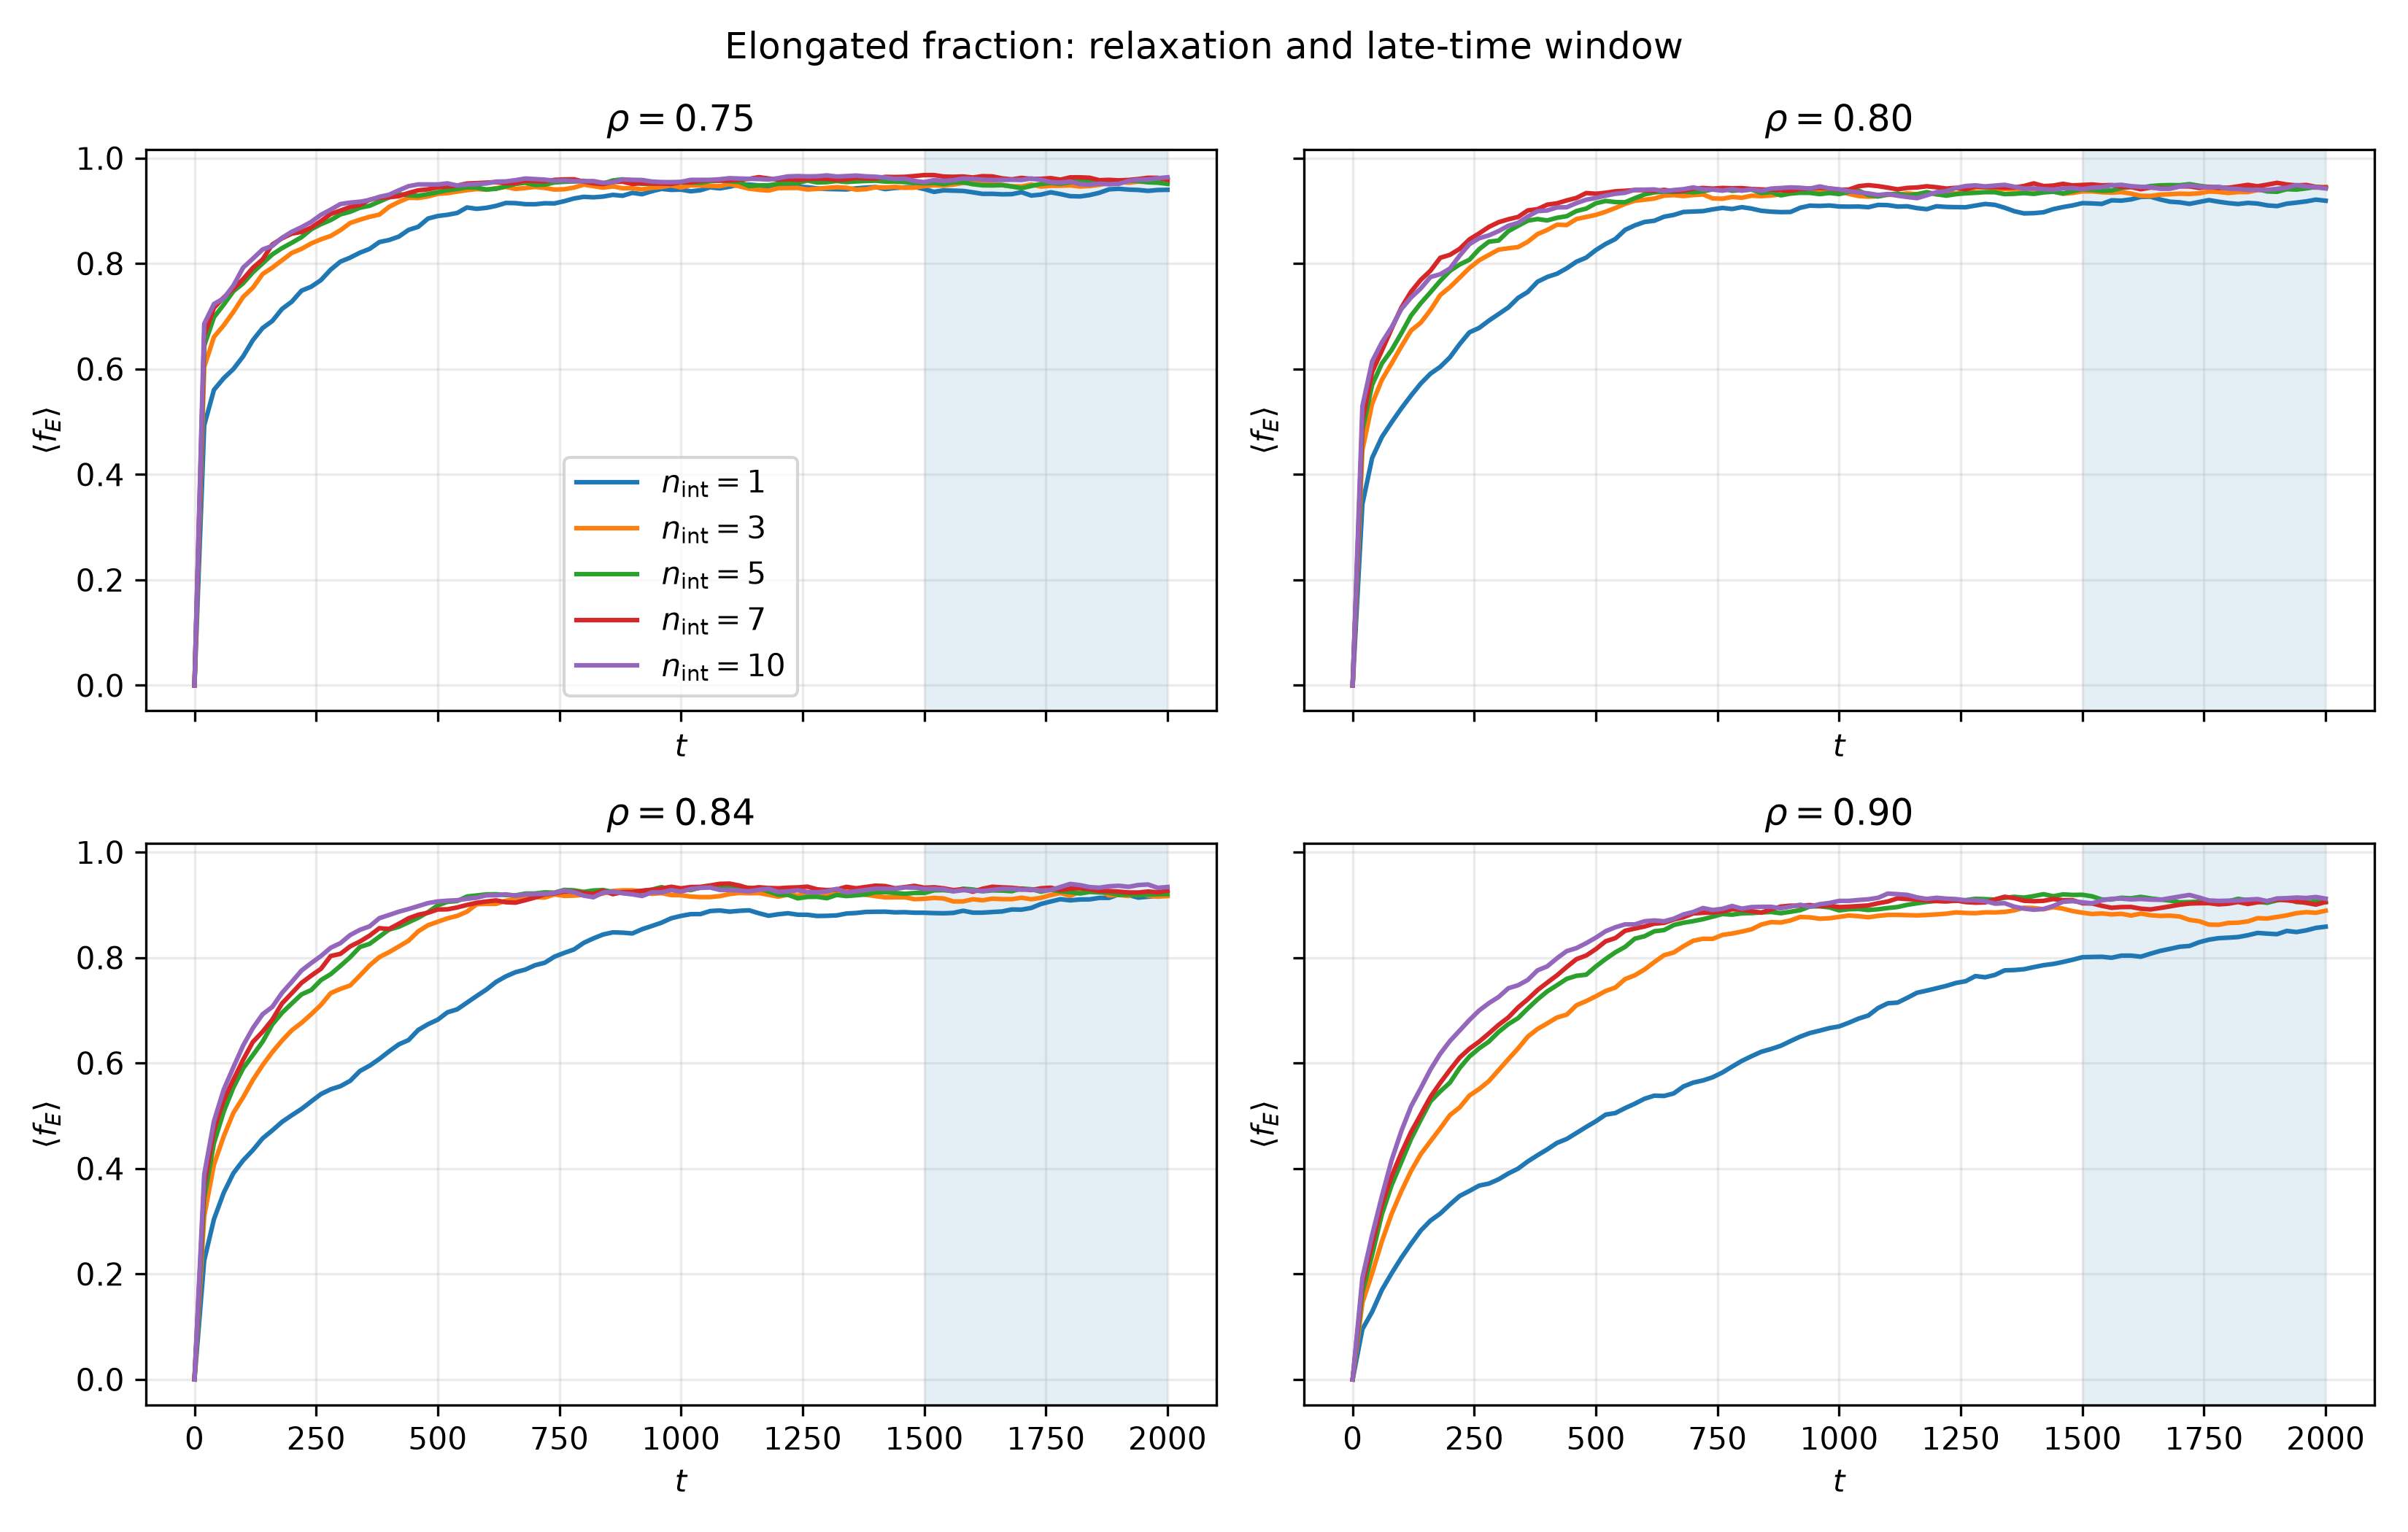
\includegraphics[width=0.9\textwidth]
    {../figures/elongated_fraction_relaxation.png}
    \caption{
        Evolución temporal de la fracción elongada para los cinco valores de
        \(n_{\rm int}\). La región sombreada corresponde a la ventana tardía
        utilizada para los promedios.
    }
    \label{fig:relaxation}
\end{figure}

Para cuantificar este comportamiento consideramos la fracción elongada
\(f_E\), el orden polar \(P\), el orden nemático \(Q\) y la fracción
\(S_{1,E}/N_E\) de células elongadas pertenecientes al mayor cluster espacial
elongado. Las medias de ensamble se muestran en la
figura~\ref{fig:macro}.

\begin{figure}[htbp]
    \centering
    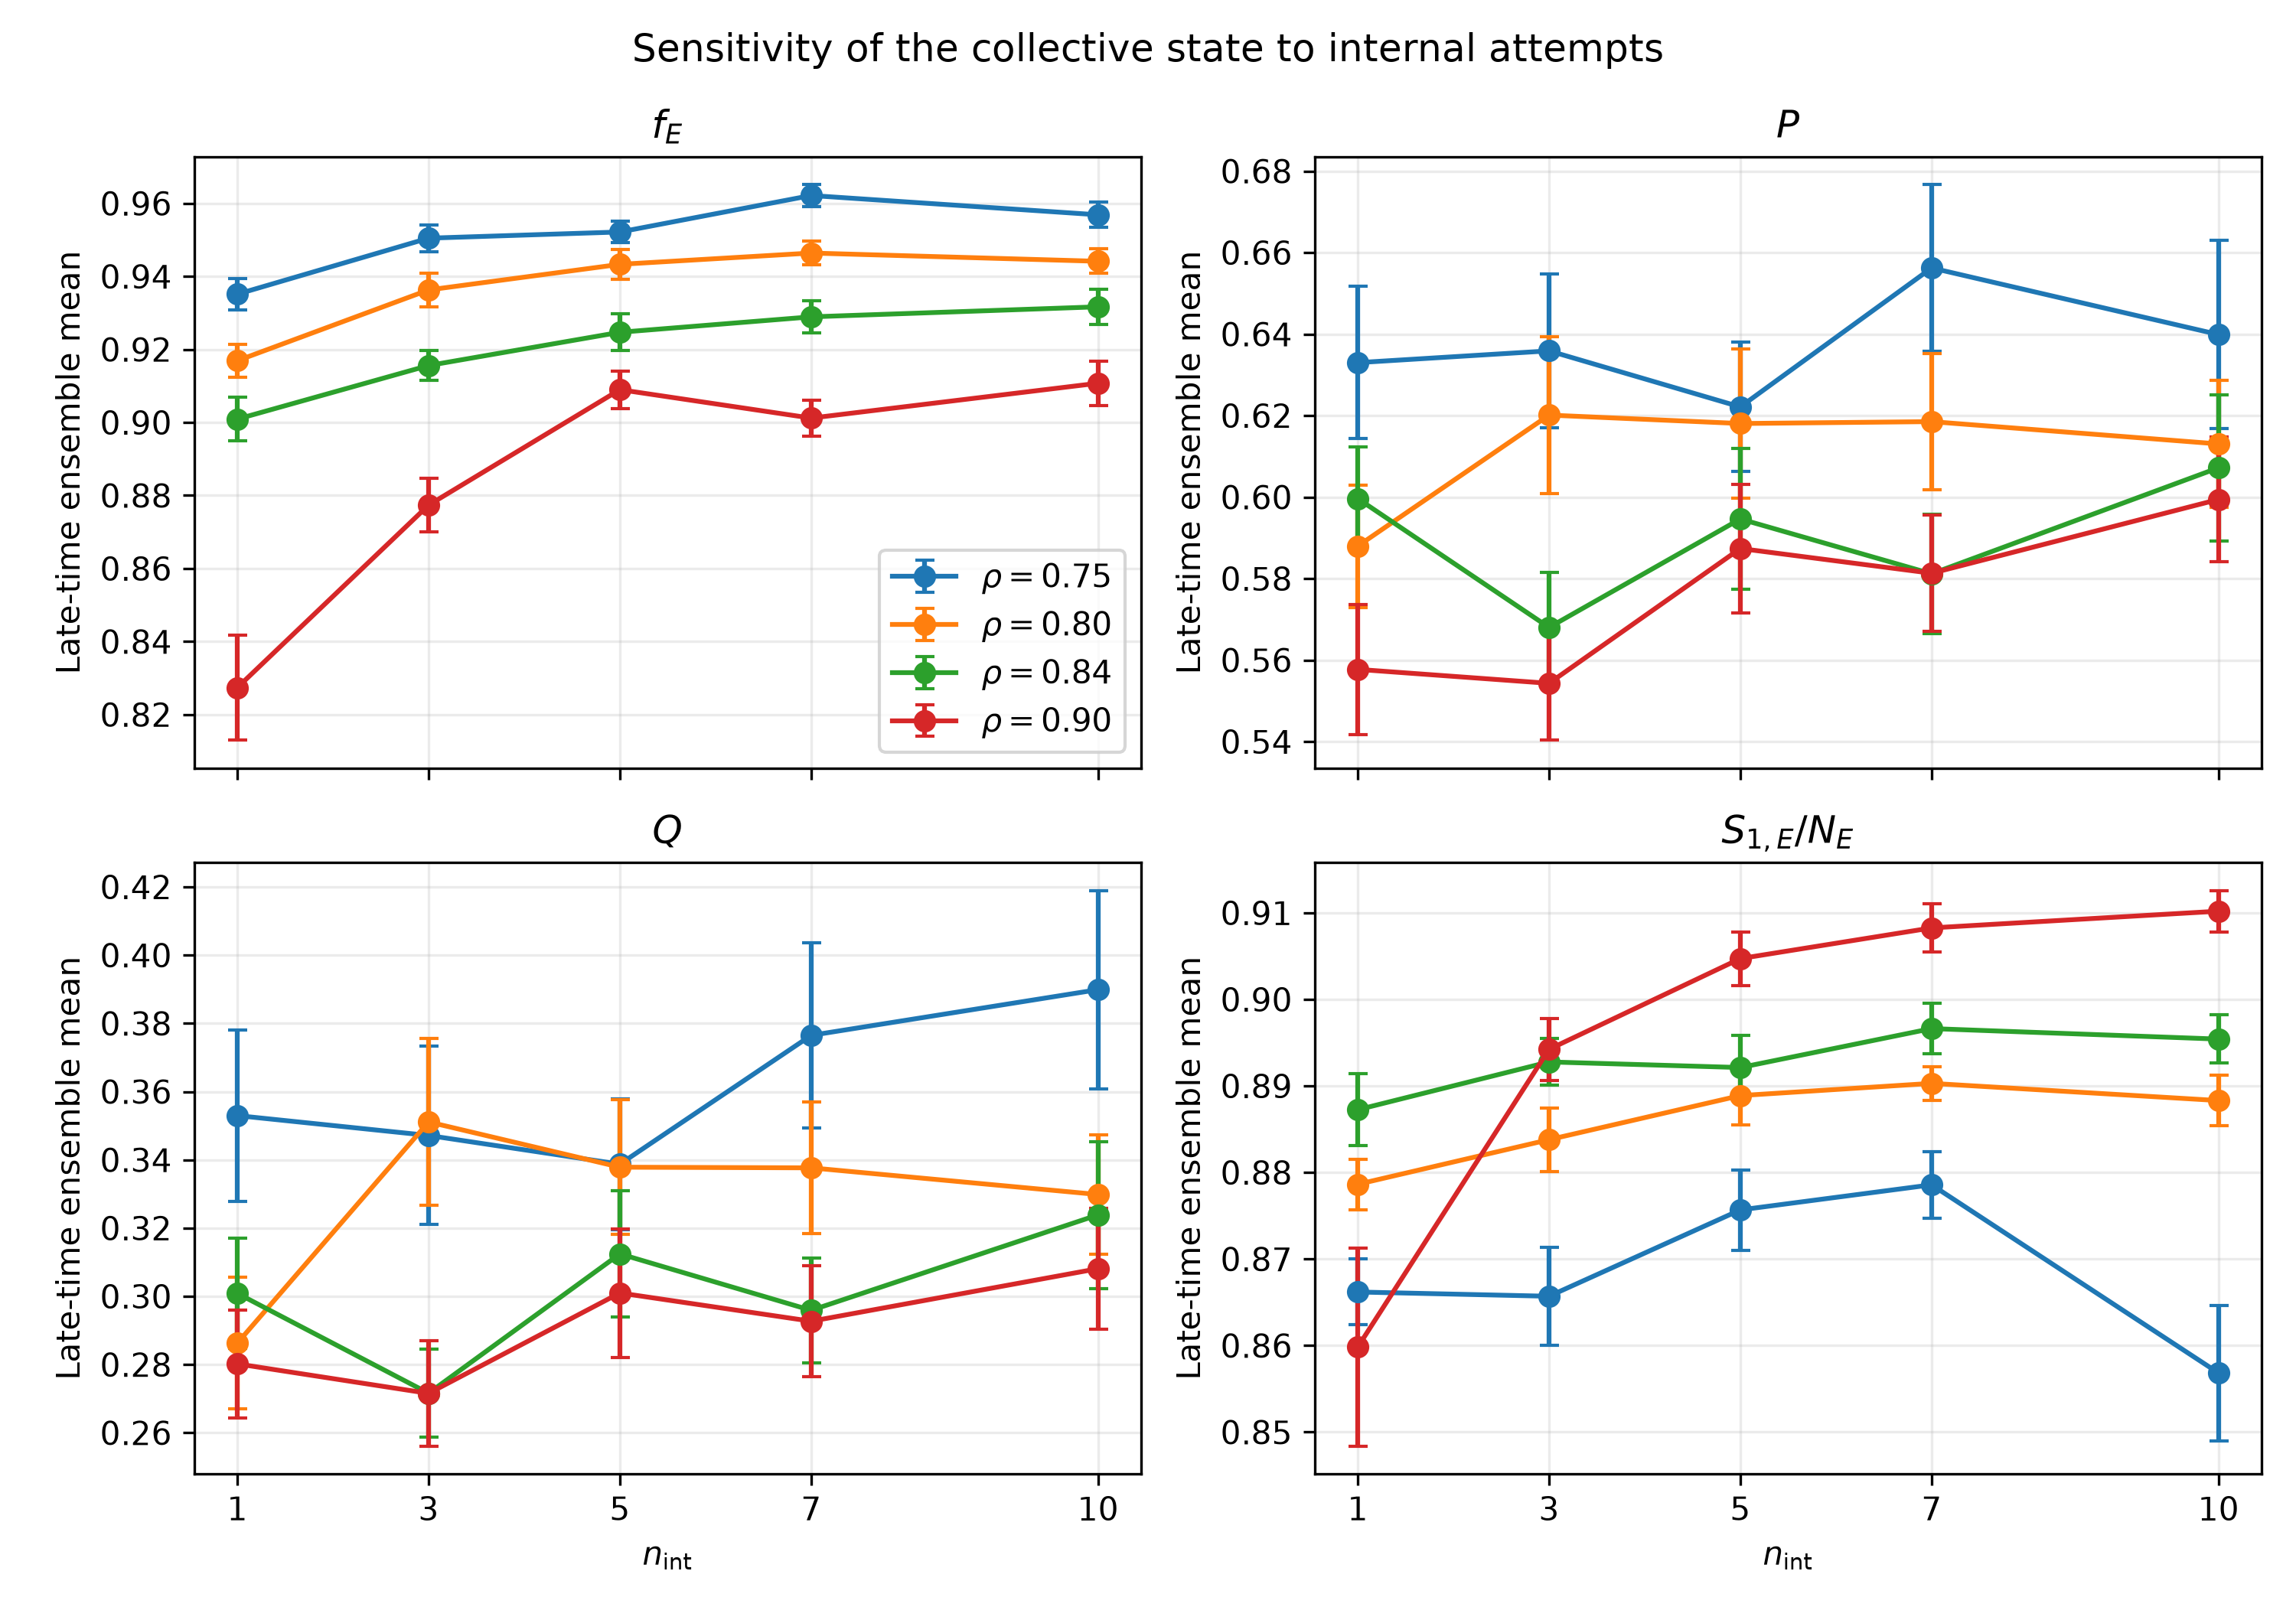
\includegraphics[width=0.9\textwidth]
    {../figures/macro_metrics_vs_n_int.png}
    \caption{
        Observables macroscópicos promediados en la ventana tardía. Las barras
        corresponden al error estándar entre las 64 realizaciones.
    }
    \label{fig:macro}
\end{figure}

La cantidad más directamente ligada a la regla de deformación, \(f_E\),
muestra una saturación clara. Tomando \(n_{\rm int}=10\) como referencia
práctica, el máximo cambio entre las cuatro densidades es

\begin{center}
\begin{tabular}{c c}
\toprule
\(n_{\rm int}\) & \(\max_{\rho}|\langle f_E\rangle_{n_{\rm int}}
-\langle f_E\rangle_{10}|\) \\
\midrule
1 & 0.083 \\
3 & 0.033 \\
5 & 0.007 \\
7 & 0.010 \\
\bottomrule
\end{tabular}
\end{center}

Por lo tanto, la variación importante ocurre entre \(1\), \(3\) y \(5\).
Los valores \(5\), \(7\) y \(10\) forman un plateau práctico en \(f_E\) y
también en la estructura de clusters elongados.

Las diferencias restantes en \(P\) y \(Q\) no disminuyen de forma monótona al
aumentar \(n_{\rm int}\). Esto indica que no observamos una deriva sistemática
hacia el resultado de \(n_{\rm int}=10\), sino fluctuaciones estadísticas de
los estados colectivos entre realizaciones.

\section{Dinámica de deformación}

También analizamos directamente los eventos de deformación. Para evitar
sesgos al promediar cocientes con diferentes denominadores, la probabilidad de
éxito de elongación se estimó de forma conjunta como

\begin{equation}
p_{\rm elong}
=
\frac{\sum_{\rm realizaciones}N_{\rm exitos}}
     {\sum_{\rm realizaciones}N_{\rm intentos}}.
\end{equation}

La figura~\ref{fig:deformation} muestra que el cambio de esta probabilidad se
reduce progresivamente y que \(n_{\rm int}=5\) ya se encuentra cerca de los
valores obtenidos para \(7\) y \(10\).

Además, en el régimen tardío la tasa de elongaciones exitosas y la tasa de
contracciones que devuelven una célula al estado redondo son prácticamente
iguales. Esto indica que la fracción elongada no corresponde a una acumulación
irreversible, sino a un balance dinámico entre ambos estados.

\begin{figure}[htbp]
    \centering
    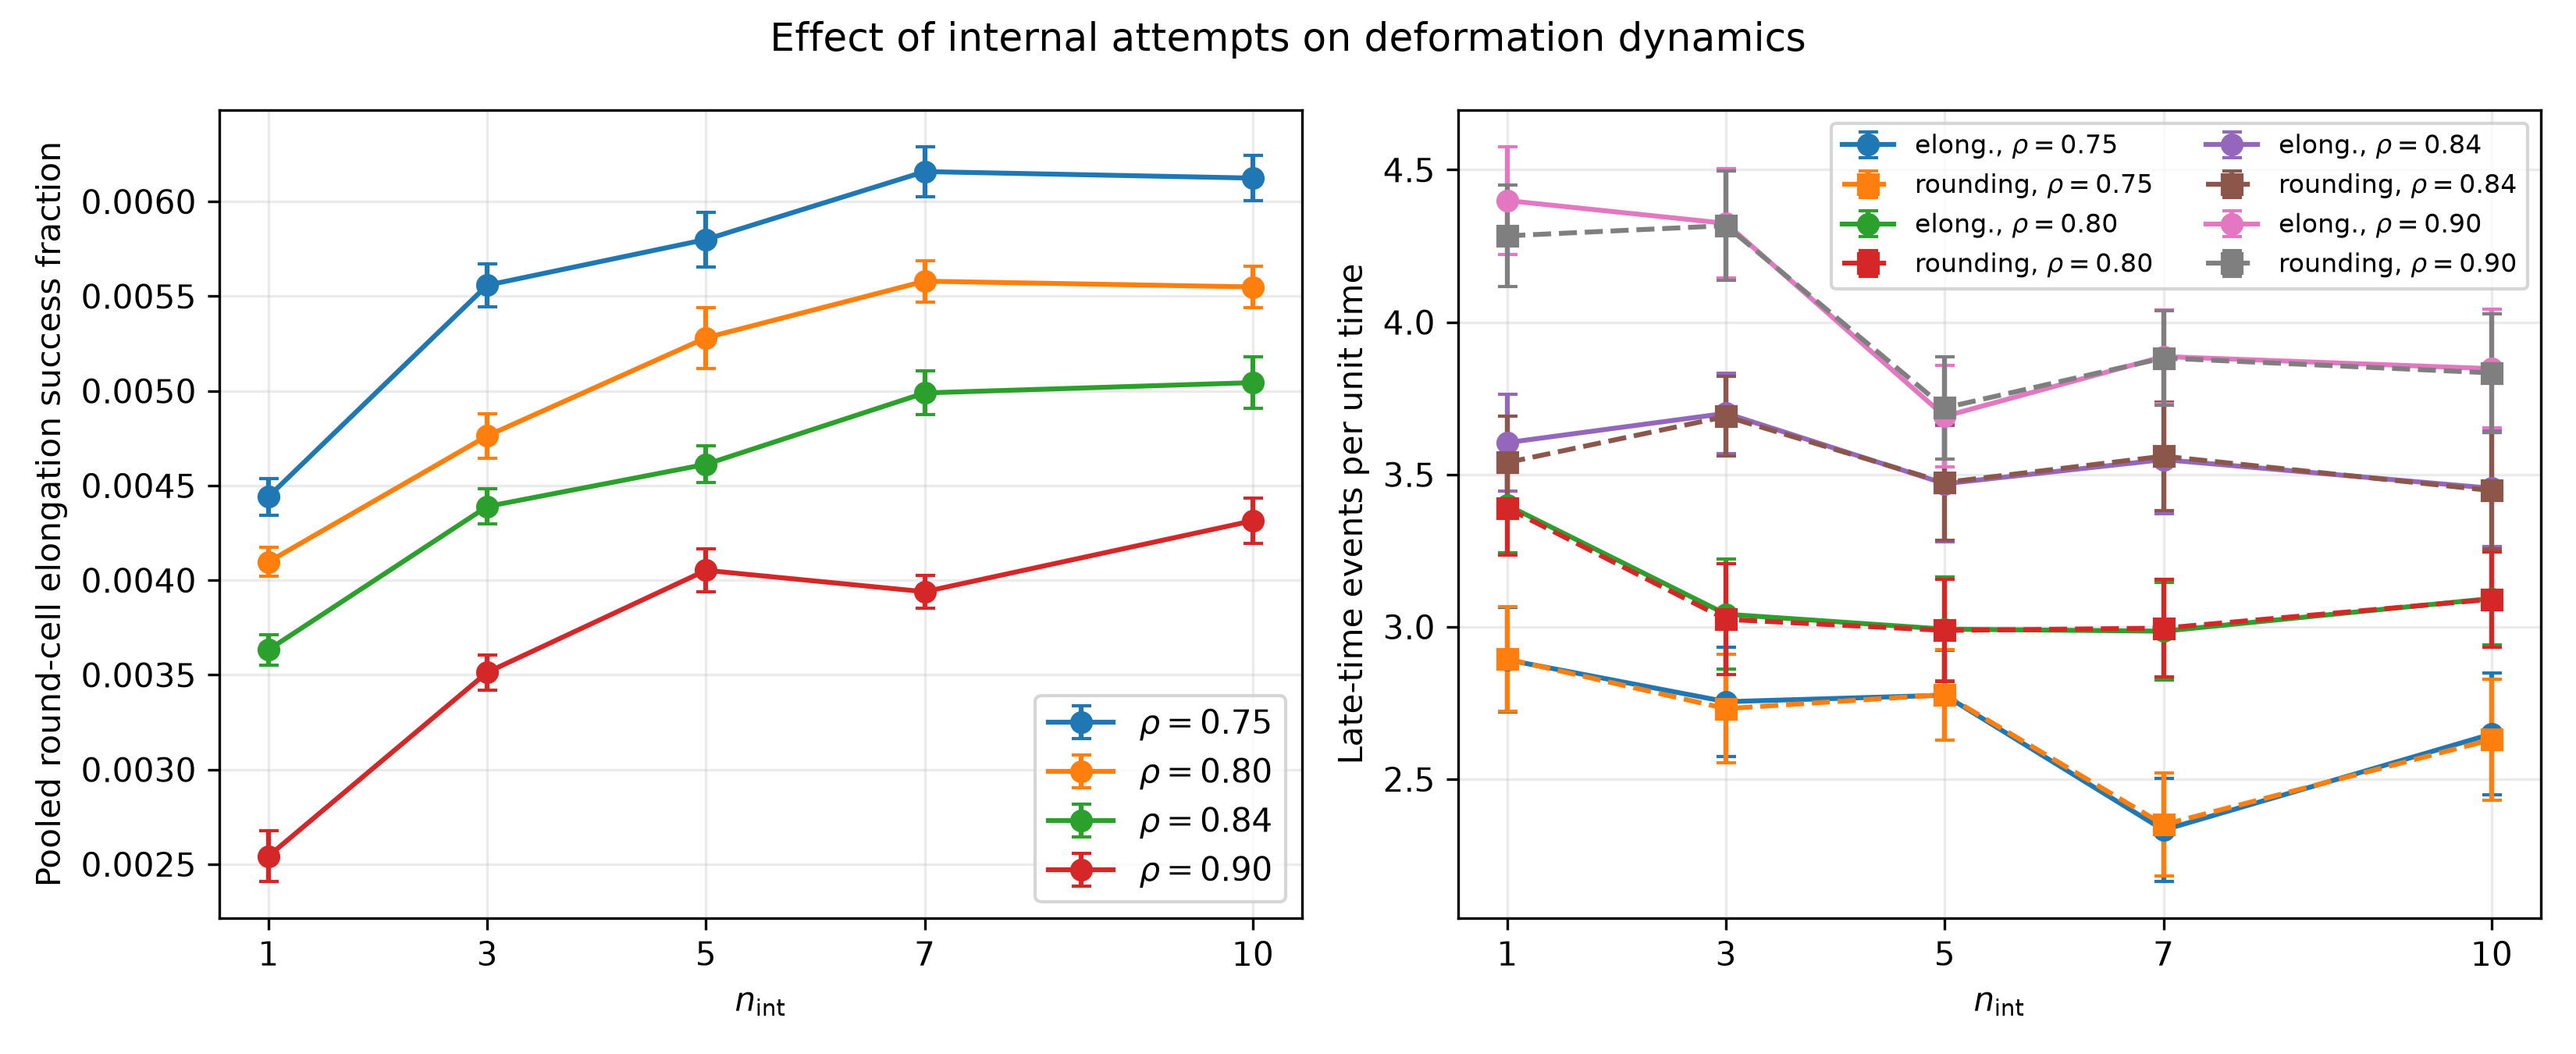
\includegraphics[width=0.9\textwidth]
    {../figures/deformation_dynamics_vs_n_int.png}
    \caption{
        Izquierda: probabilidad conjunta de éxito de elongación.
        Derecha: tasas de elongación exitosa y de contracción al estado
        redondo. En el régimen tardío ambas tasas se encuentran casi
        balanceadas.
    }
    \label{fig:deformation}
\end{figure}

\section{Controles microscópicos}

Finalmente verificamos que la elección de \(n_{\rm int}\) no introduzca un
cambio no deseado en la dinámica microscópica. La
figura~\ref{fig:sanity} muestra el percentil 95 de la máxima superposición
normalizada y el percentil 95 de la velocidad instantánea.

Ambas cantidades permanecen esencialmente en el mismo régimen para todos los
valores estudiados. El percentil 95 de la superposición se mantiene alrededor
de \(0.79\), no se observan eventos con \(\xi_{\max}>0.95\), y la fracción de
contracciones rechazadas por la regla de seguridad permanece aproximadamente
por debajo del \(1\%\). Tampoco aparecen velocidades anómalas al aumentar
\(n_{\rm int}\).

\begin{figure}[htbp]
    \centering
    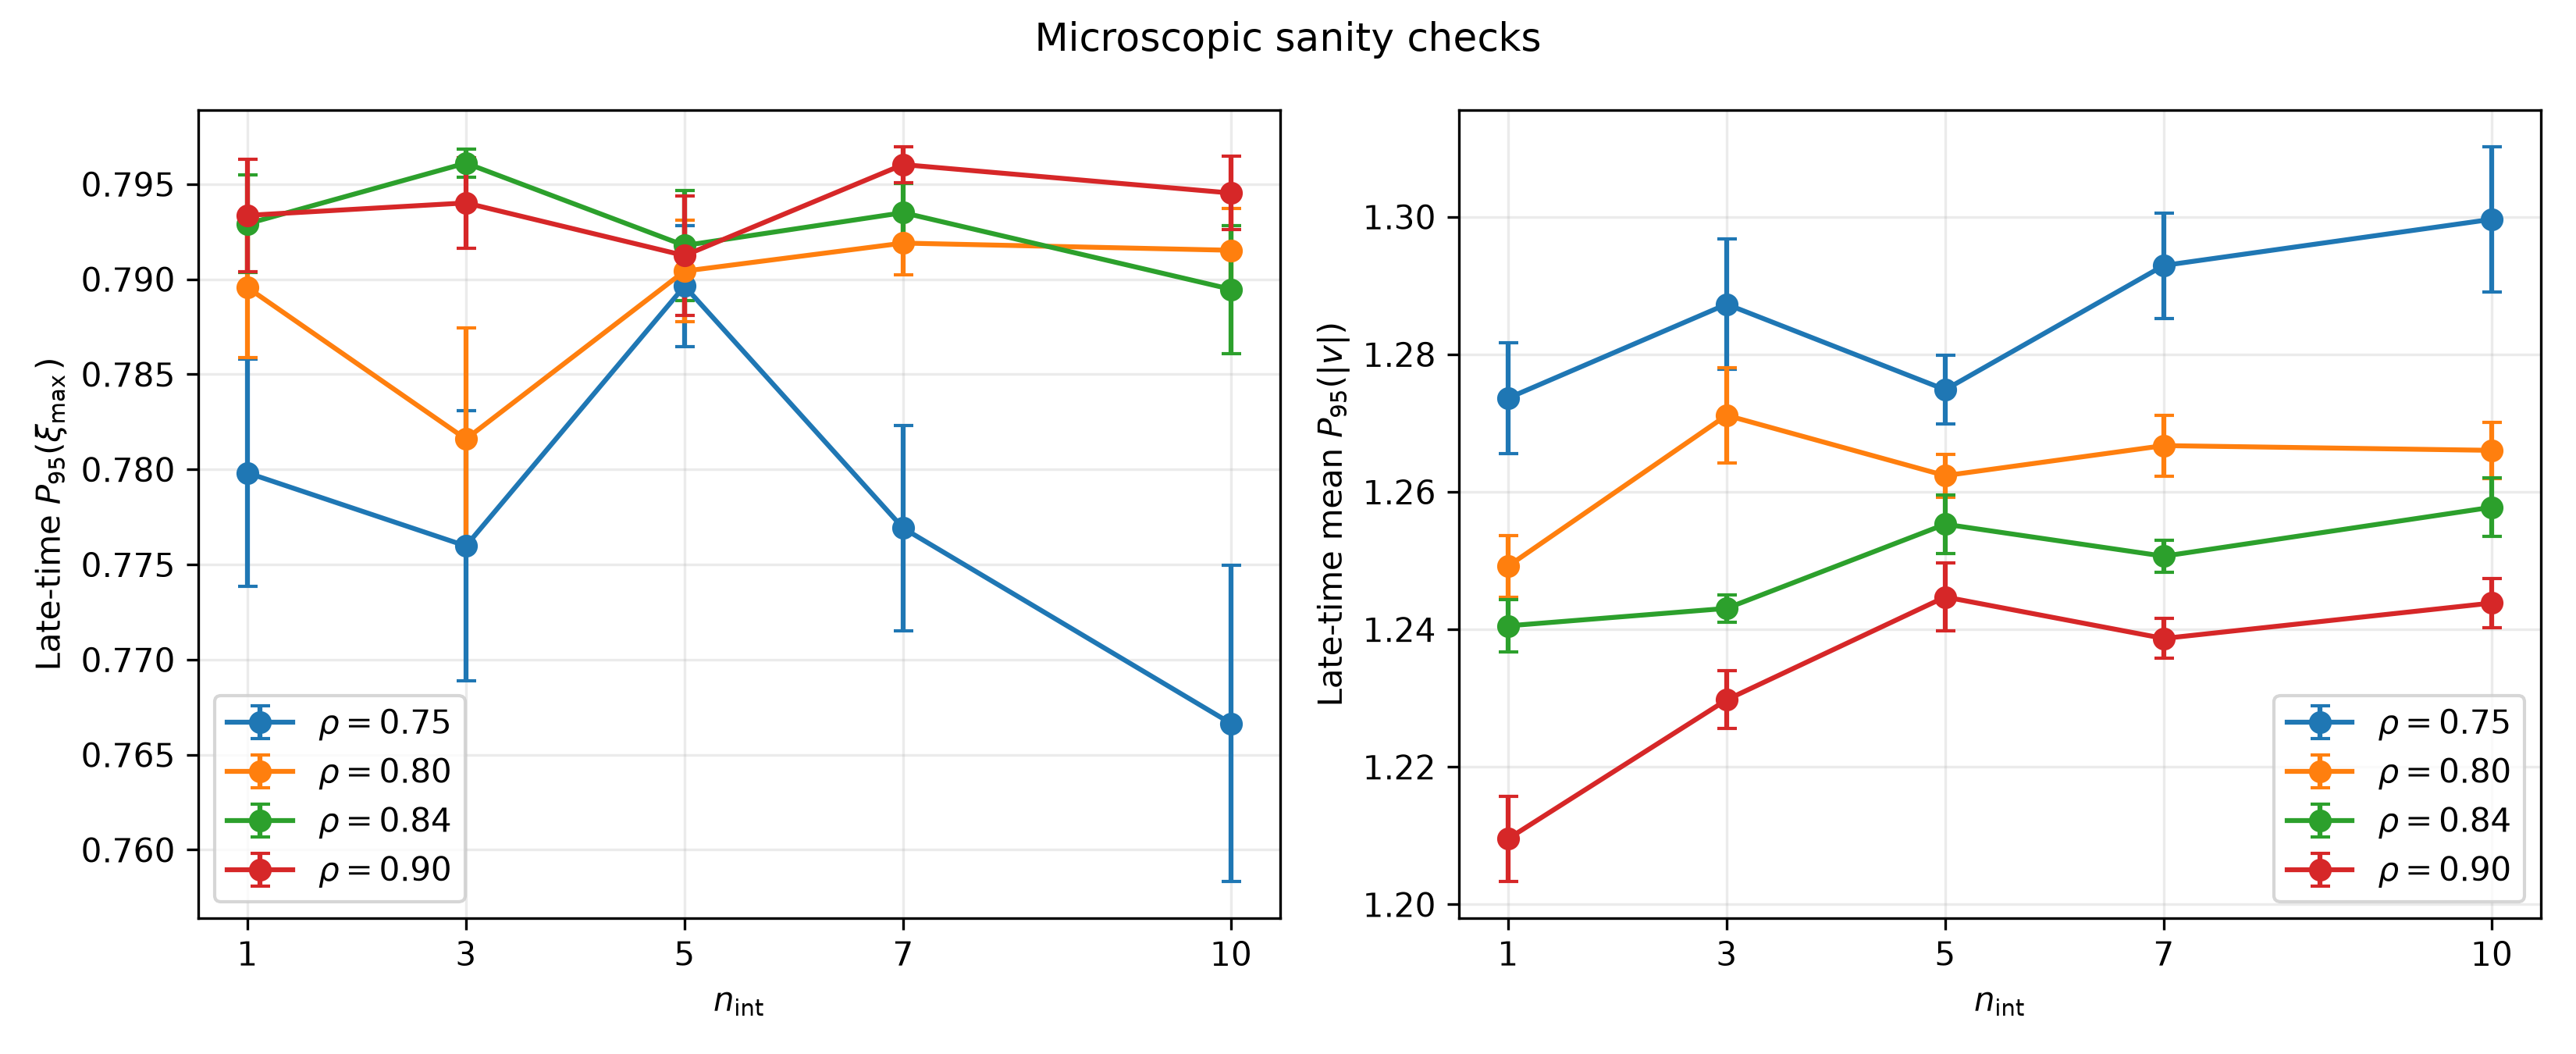
\includegraphics[width=0.9\textwidth]
    {../figures/microscopic_sanity_checks.png}
    \caption{
        Controles microscópicos en la ventana tardía: superposición máxima y
        cola de la distribución de velocidades instantáneas.
    }
    \label{fig:sanity}
\end{figure}

\section{Elección de \texorpdfstring{\(n_{\rm int}\)}{nint}}

Los resultados permiten distinguir tres situaciones:

\begin{itemize}
    \item \(n_{\rm int}=1\): el número de orientaciones probadas es
    insuficiente y modifica de manera clara el estado colectivo;
    \item \(n_{\rm int}=3\): captura la mayor parte del efecto, pero todavía
    se observan diferencias, principalmente en el régimen de mayor densidad;
    \item \(n_{\rm int}\geq5\): los observables directamente ligados a la
    deformación entran en un plateau práctico y los controles microscópicos
    permanecen estables.
\end{itemize}

Elegimos entonces el menor valor dentro de este plateau:

\begin{equation}
\boxed{n_{\rm int}=5},
\end{equation}

que en la implementación corresponde a

\begin{equation}
\boxed{\texttt{cell\_max\_def\_attempts}=5}.
\end{equation}

No interpretamos esta elección como una convergencia matemática en
\(n_{\rm int}\), sino como una validación de robustez del modelo: aumentar el
número de orientaciones de \(5\) a \(7\) o \(10\) no produce cambios
sistemáticos relevantes en el estado colectivo, mientras que sí aumenta el
costo de cada intento de elongación.

\section{Conclusión}

La campaña permite cerrar el número de intentos internos de elongación en

\begin{equation}
\boxed{n_{\rm int}=5}.
\end{equation}

Con \(\lambda_{\rm core}=1\), \(\Delta t=0.01\) y
\(n_{\rm int}=5\) ya fijados, el siguiente parámetro a validar es el período
entre barridos de deformación \(T_{\rm def}\). Finalmente se revisará el
umbral de seguridad de contracción \(\xi_{\rm safe}\).

\end{document}
